\section{Fundamentação Teórica}
\subsection{Prosódia}

\begin{frame}{Prosódia}
  \begin{block}{Definição de Prosódia}<1->
    Prosódia é o estudo dos aspectos \textbf{entoacionais}, \textbf{rítmicos} e
    \textbf{enfáticos} da linguagem \cite{lang_processing_book}.
  \end{block}
  \begin{block}{}<2->
    % TEM QUE TER A PÁGINA: 20
    \begin{displayquote}[\citeauthor{prosodia_plinio_barbosa_book}:20
      \cite{prosodia_plinio_barbosa_book}]
      (\dots) o estudo da prosódia não considera diretamente o conteúdo segmental, ou
      \textbf{o que se diz}, e sim a forma sonora e sua função ligadas ao
      \textbf{como se diz}.
    \end{displayquote}
  \end{block}
  \begin{block}{}<3->
    A prosódia tem seu campo de estudo nos domínios \textbf{linguístico},
    \textbf{paralinguístico} e \textbf{extralinguístico}.
  \end{block}
\end{frame}

\begin{frame}{Prosódia}
  \setbeamercolor{caption}{bg=white}

  \setbeamertemplate{caption}{
    \begin{beamercolorbox}[wd=\linewidth, center, sep=1pt]{caption}
      \tiny
      {\usebeamercolor[fg]{caption name}\insertcaptionname:} \insertcaption
    \end{beamercolorbox}
  }

  \begin{figure}
    \centering
    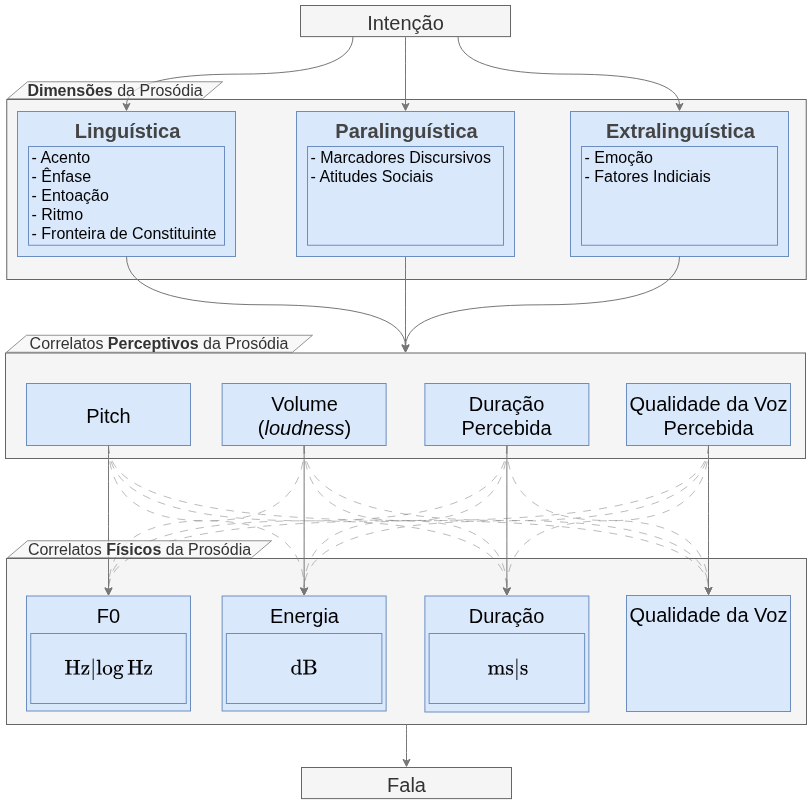
\includegraphics[width=0.5\linewidth]{imgs/DiaTTS-Toolkit-Prosody.png}
    \caption{Fluxo \textit{top-down} da materialização da fala, desde a cognição
      (\textbf{intenção}) até a materialidade (\textbf{o som/fala})
      \cite{prosodia_plinio_barbosa_book}\cite{Prosodia_Barbosa_2012}. Fonte: Elaborada
    pelo autor.}
    % \fautor
  \end{figure}
\end{frame}

% \begin{frame}{Prosódia}
% \begin{figure}
%   \centering
%   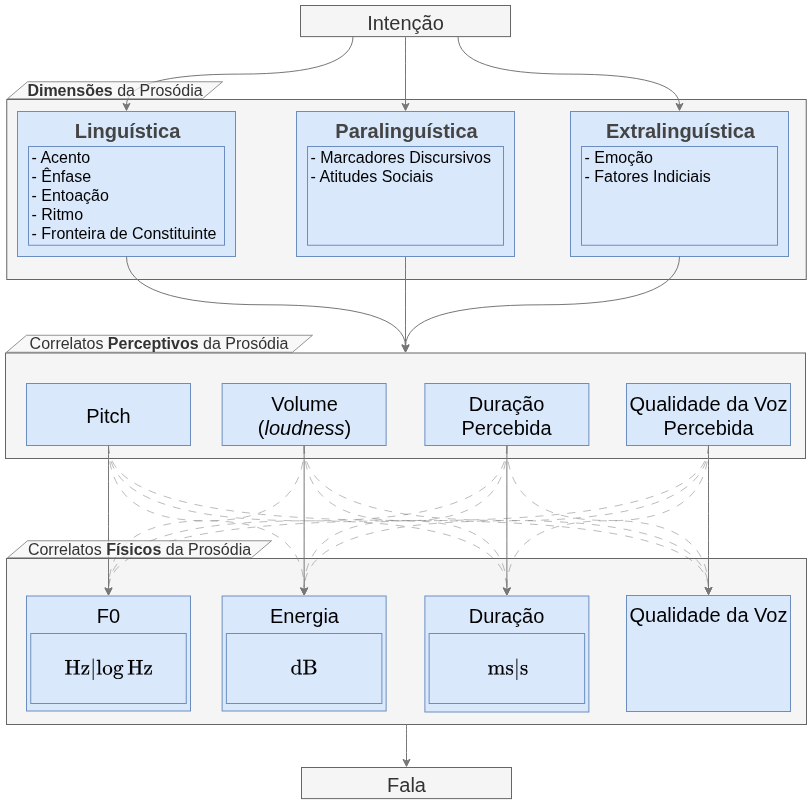
\includegraphics[width=0.6\linewidth]{imgs/DiaTTS-Toolkit-Prosody.png}
%   % \fautor
% \end{figure}
% \end{frame}

\begin{frame}{Prosódia}{Unidades Prosódicas}
  \begin{block}{}
    \begin{itemize}
      \item Fonologia \(\to\) fonema.
      \item Morfologia \(\to\) morfema.
      \item Prosódia \(\to\) \dots
    \end{itemize}
  \end{block}
\end{frame}

\begin{frame}{Prosódia}{Unidades Prosódicas}
  \begin{block}{}
    \begin{displayquote}[\customcite{prosodia_plinio_barbosa_book}:37
      \cite{prosodia_plinio_barbosa_book}]
      A prosódia é o componente de nossa fala que \textbf{organiza} nossos enunciados,
      moldando nossa maneira de falar através do concurso de modificações articulatórias
      que se manifestam acusticamente em \textbf{unidades prosódicas}.
    \end{displayquote}
  \end{block}
\end{frame}

\begin{frame}{Prosódia}{Unidades Prosódicas}
  \begin{block}{Organização Hierárquica \cite{prosodia_plinio_barbosa_book}}
    \begin{enumerate}
      \item Sílaba
      \item Pé
      \item Palavra fonológica/prosódica
      \item Unidade entoacional
      \item Enunciado
    \end{enumerate}
  \end{block}
\end{frame}

\begin{frame}{Prosódia e Discurso}{Tomada de Turno}
  \begin{figure}
    \centering
    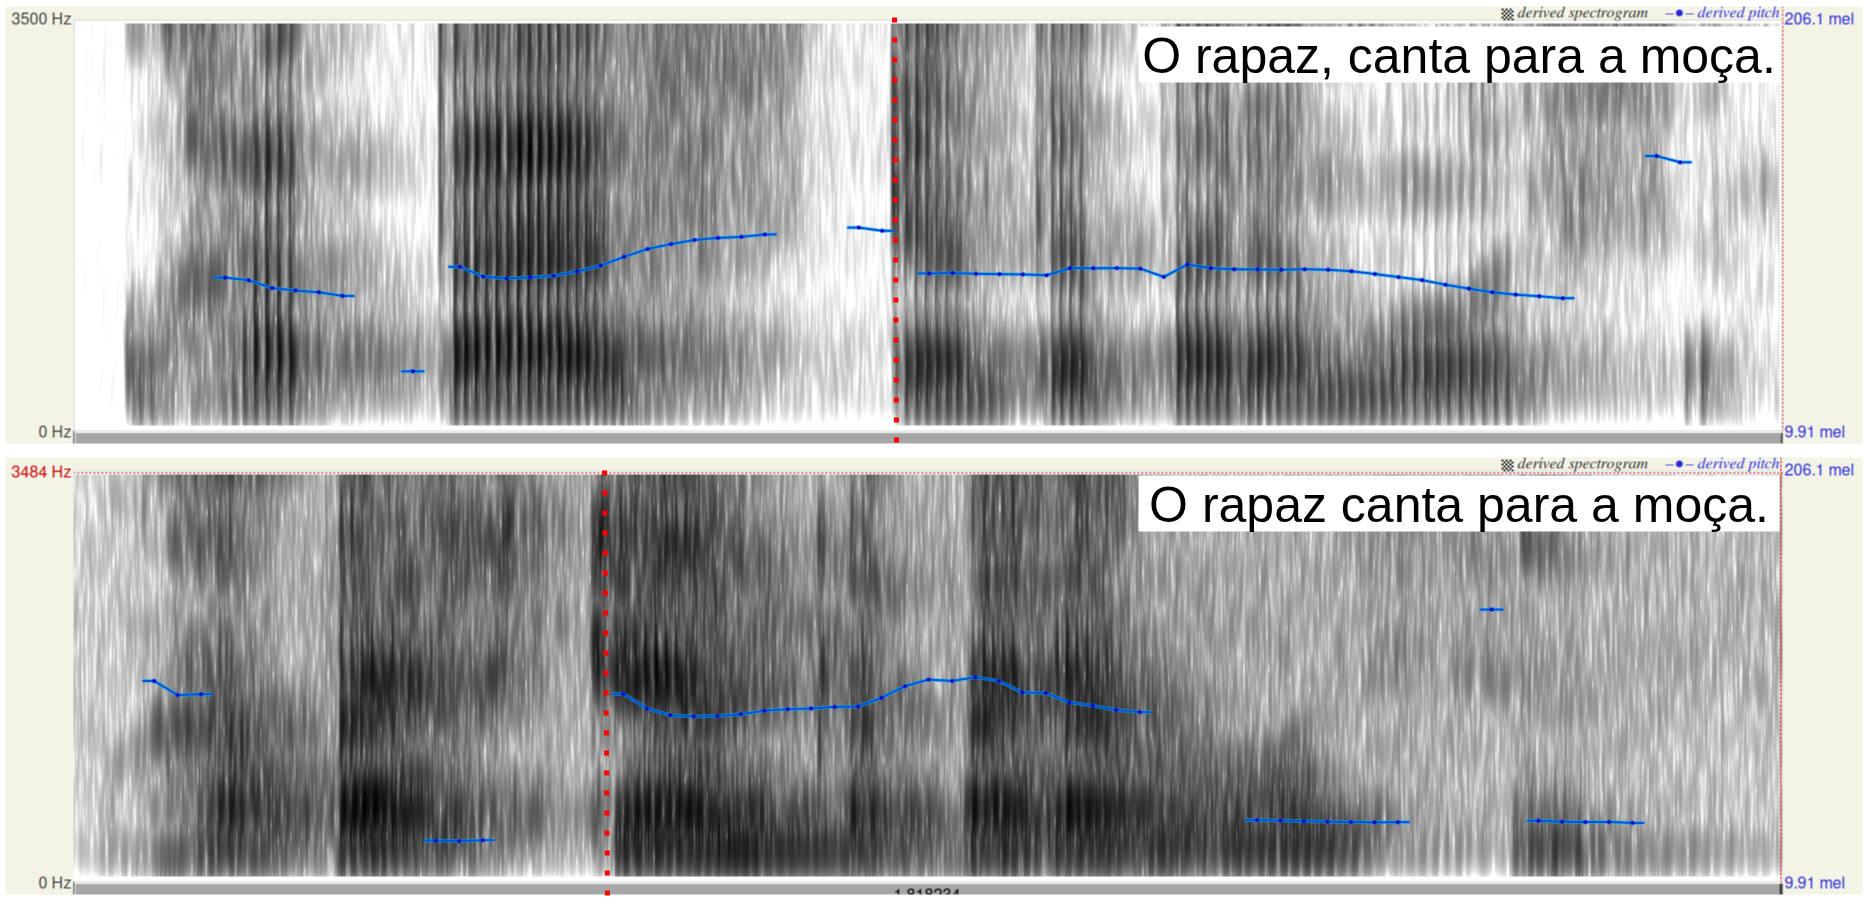
\includegraphics[width=0.9\linewidth]{imgs/DiaTTS-Toolkit-SintagmaEntoacional.png}
    \caption{\textbf{Unidade Entoacional}: fronteira terminal.}
    \label{fig:UnidadeEntoacional}
  \end{figure}
\end{frame}

%Estudo da Fala-em-interação  (Análise da Conversa,  2009)
% Referenciar!
\subsection{Conversação}
\begin{frame}{Turnos}
  \begin{block}{Diálogo como sequência de turnos.}
    Um diálogo $\mathcal{D}$ é uma sequência de $n$ turnos \cite{lang_processing_book}
    \[
      \mathcal{D} = (t_0, t_1, \dots, t_{n-1})
    \]
  \end{block}
  \begin{block}{}
    Cada turno $t_i$ pertence a um falante, de modo que turnos adjacentes pertencem a
    falantes diferentes.
    \[
      t_i \in \mathbb{S}_k \implies (t_{i-1}, t_{i+1}) \notin \mathbb{S}_k
    \]
    \(\mathbb{S}_k\) é o conjunto de turnos do falante \(k\).
  \end{block}
\end{frame}

\begin{frame}{Atos de Fala}
  \begin{block}{}
    Cada enunciado (\textit{utterance}) num diálogo pode ser visto como uma \textbf{ação}
    sendo performada pelo falante.
  \end{block}
  \begin{block}{Taxonomia dos Atos}
    Não existe uma única maneira de classificar os \textbf{atos de fala}. \\
    A classificação a seguir está no livro \textit{Speech Acts: An Essay in the
    Philosophy of Language. Searle, J. R. (1969)}\cite{SpeechActs_Searle1969_book}.
    \begin{multicols}{2}
      \begin{itemize}
        \item Requisição
        \item Afirmação
        \item Questionamento
        \item Agradecimento
        \item Aconselhamento
        \item Aconselhamento
        \item Saudação
        \item Parabenização
      \end{itemize}
    \end{multicols}
  \end{block}
\end{frame}

\begin{frame}{\textit{Grounding}}
  \begin{block}{}
    Os atos da fala não agem de maneira independente; pelo contrário, são uma
    \textbf{tarefa coletiva} \cite{lang_processing_book}.
  \end{block}
  \begin{block}{}
    Desta forma, os participantes do diálogo buscam uma \textbf{base de entendimento
    comum} (\textit{grounding}) na qual todos concordam, e o diálogo constrói-se a partir
    daí \cite{lang_processing_book}.
  \end{block}
\end{frame}

\begin{frame}{\textit{Grounding}}
  \begin{block}{Contribuição}
    Cada ato de fala adjacente constitui uma \textbf{contribuição}
    \cite{contributing_to_discourse_1989}. \\
    Cada contribuição tem duas fases:
    \begin{itemize}
      \item \textbf{Apresentação}: O falante \(\mathbb{S}_A\) apresenta o enunciado \(u\)
        sob a suposição de que, se o ouvinte \(\mathbb{S}_B\) fornecer evidência \(e\),
        ele poderá acreditar que \(u\) foi compreendido.
      \item \textbf{Aceitação}: O ouvinte \(\mathbb{S}_B\) aceita \(u\) fornecendo a
        evidência \(e'\) \textit{do que ele acredita} que entendeu. Ele o faz assumindo
        que, uma vez que  \(\mathbb{S}_A\) registra a evidência \(e'\), ele acredita que
        foi compreendido.
    \end{itemize}
    \pause
    As fases da contribuição, de \textbf{forma cíclica}, constituem o entendimento mútuo
    (\textit{grounding}).
  \end{block}
\end{frame}

\begin{frame}{\textit{Grounding}}
  \begin{block}{Evidências de Entendimento}
    Evidências de entendimento\cite{contributing_to_discourse_1989} ordenadas das mais
    fracas para as mais fortes:
    \begin{enumerate}
      \item \textbf{Atenção Continuada} (\textit{Continued Attention}).
      \item \textbf{Próxima Contribuição Relevante} (\textit{Relevant Next Contribution}).
      \item \textbf{Reconhecimento/Sinais} (\textit{Acknowledgement}) --
        pausas-preenchidas (\textit{filling-gaps}).
      \item \textbf{Demonstração/Paráfrase} (\textit{Demonstration}).
      \item \textbf{Exibição/Repetição literal} (\textit{Display}).
    \end{enumerate}
  \end{block}
\end{frame}

\begin{frame}{Estrutura do Diálogo}
  \begin{block}{}
    \begin{itemize}
      \item \textbf{Subdiálogo}: \textbf{estrutura local} entre atos de fala.
      \item \textbf{Diálogo}
    \end{itemize}
  \end{block}
  \pause
  \begin{block}{}
    Correlaciona-se com o entendimento de \textit{coerência local} e \textit{coerência
    global} \cite{lang_processing_book}.
  \end{block}
\end{frame}

\begin{frame}{Iniciativa}
  \begin{block}{}
    Às vezes uma conversa é completamente controlada por um único participante, como no
    caso de \textbf{entrevistas}.
  \end{block}
  \pause
  \begin{block}{Iniciativa}
    O conceito de iniciativa (\textit{conversational initiative}) refere-se ao
    \textbf{controle} e ao \textbf{direcionamento} do fluxo de uma conversa. Em termos
    simples, ter a iniciativa significa ser quem está \textit{conduzindo} o diálogo
    naquele momento -- seja fazendo as perguntas, introduzindo novos tópicos ou exigindo
    uma resposta da outra parte  \cite{lang_processing_book}.
  \end{block}
\end{frame}

\begin{frame}{Prosódia e Discurso}
  \begin{block}{}
    \begin{itemize}
      \item Prosódia e discurso são intimamente relacionados.
        \pause
      \item É através da \textbf{análise prosódica} que identificamos as características
        intrínsecas ao diálogo...
    \end{itemize}
  \end{block}
\end{frame}

\begin{frame}{Prosódia e Discurso}{Tomada de Turno}
  \begin{block}{Definição}
    Tomada de turno (\textit{turn-taking}) refere-se ao sistema de sinalizações e regras
    que permitem aos falantes alternarem quem está falando de forma fluida e organizada
    \cite{Prosodia_Barbosa_2012} \cite{prosodia_plinio_barbosa_book}.
  \end{block}
\end{frame}

\begin{frame}{Prosódia e Discurso}{Tomada de Turno}
  \begin{block}{Tomada de Turno \textbf{Cooperativa}}
    Acontece quando as regras de passagem de turno são respeitadas -- ao final de uma
    interrogação, por exemplo. Neste cenário, \textbf{unidades prosódicas} específicas
    sinalizam que o primeiro interlocutor acabou seu turno e está passando a vez para o
    segundo interlocutor.
  \end{block}
\end{frame}

\begin{frame}{Prosódia e Discurso}{Tomada de Turno}
  \begin{block}{Tomada de Turno \textbf{Competitiva}}
    Acontece quando as regras de passagem de turno não são respeitadas, como em casos de
    \textbf{interrupções}. Neste cenário, um interlocutor, diferente do que está falado
    (i.e. do que \textit{detém} o turno), utiliza de artifícios prosódicos (e.g. aumenta
    a intensidade da fala), para roubar o turno.
  \end{block}
\end{frame}

\begin{frame}{Prosódia e Discurso}{Tomada de Turno}
  \begin{figure}
    \centering
    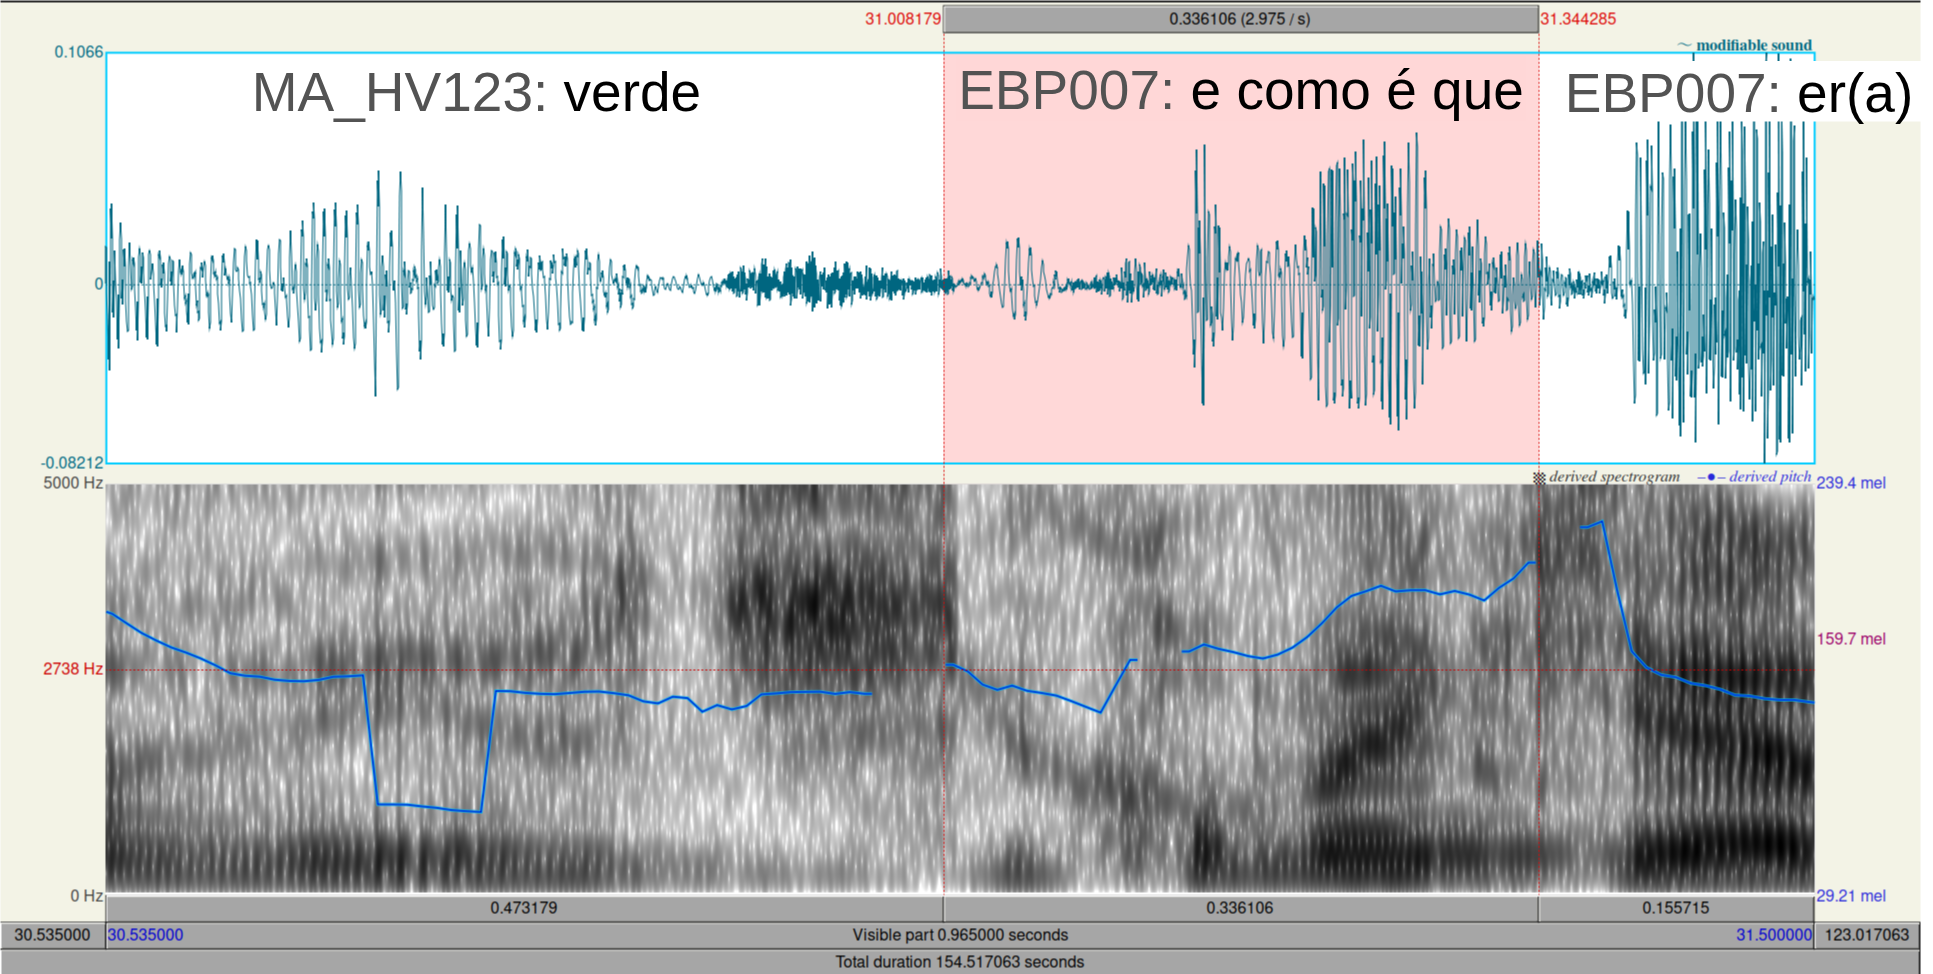
\includegraphics[width=0.8\linewidth]{imgs/DiaTTS-Toolkit-Interruption.png}
    \caption{Espectrograma demonstrando a tomada de turno em um segmento do MuPeTalk.}
    \label{fig:interruption}
  \end{figure}
\end{frame}

\begin{frame}{Prosódia e Discurso}{Formas Prosódicas}
  \begin{block}{}
    A prosódia direciona diferentes \textbf{ilocuções}, i.e., a intenção da ação na fala:
    uma ordem, uma dúvida, um convite, um chamado, etc.
  \end{block}
  \pause
  \begin{block}{Definição}
    \textbf{Formas Prosódicas} são as configurações acústico-articulatórias dinâmicas e
    contínuas que constituem a materialização física da prosódia em um enunciado
    \cite{prosodia_plinio_barbosa_book}.
  \end{block}
\end{frame}

\begin{frame}{Prosódia e Discurso}{Formas Prosódicas}
  \begin{block}{Entrainment Prosódico}
    Definido pela capacidade dos seres humanos se ajustarem, tanto em nível
    comportamental como discursivo, ao seu interlocutor \cite{ProsodicEntrainment}.
  \end{block}
\end{frame}

\subsection{Modelos de TTS}

\begin{frame}{Tipos de modelos de \textit{TTS}}{Não-Controláveis vs.\ Controláveis}
  \begin{block}{Controlabilidade}
    % Capacidade de um modelo de síntese de fala de \textbf{controlar explicitamente}
    % atributos prosódicos da fala.\cite{Survey-ControllableSpeechSynthesis}
    Capacidade de um modelo de síntese de fala de \textbf{controlar explicitamente} os
    correlatos físicos ou perceptivos da prosódia \cite{Survey-ControllableSpeechSynthesis}.
  \end{block}
  \begin{block}{}
    Desta forma:
    \begin{itemize}
      \item \textbf{Modelos Não-Controláveis}: não contêm estruturas dedicadas à
        controlar atributos fonéticos.
      \item \textbf{Modelos Controláveis}: contêm estruturas dedicadas à controlar
        atributos prosódicos.
    \end{itemize}
  \end{block}
\end{frame}

\begin{frame}{Tipos de modelos de \textit{TTS}}{Não-Controláveis vs.\ Controláveis}
  \setbeamercolor{caption}{bg=white}

  \setbeamertemplate{caption}{
    \begin{beamercolorbox}[wd=\linewidth, center, sep=2pt]{caption}
      {\usebeamercolor[fg]{caption name}\insertcaptionname:} \insertcaption
    \end{beamercolorbox}
  }

  \begin{figure}
    \centering
    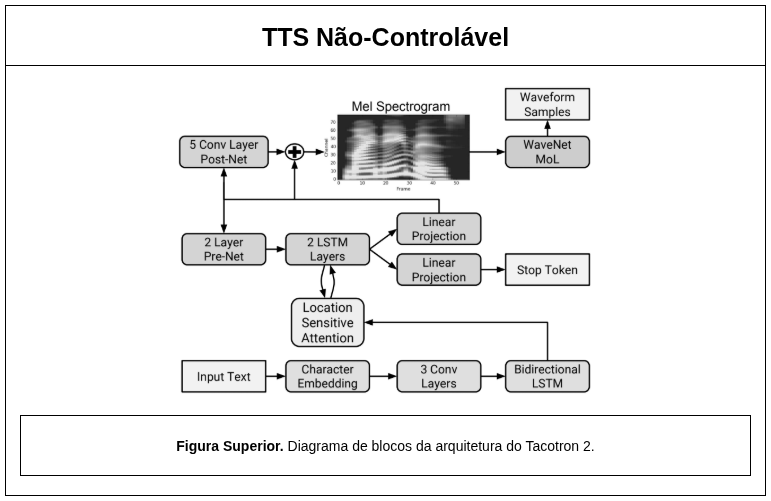
\includegraphics[width=0.7\linewidth]{imgs/DiaTTS-Toolkit-UnControllable.png}
    \caption{Arquitetura do \textit{Tacotron2}, modelo autorregressivo (\textit{AR})
    baseado em \textit{RNN} -- Adaptado de \cite{Tacotron2}.}
    \label{fig:uncontrollable}
  \end{figure}
\end{frame}

\begin{frame}{Tipos de modelos de \textit{TTS}}{Não-Controláveis vs.\ Controláveis}
  \setbeamercolor{caption}{bg=white}

  \setbeamertemplate{caption}{
    \begin{beamercolorbox}[wd=\linewidth, center, sep=2pt]{caption}
      {\usebeamercolor[fg]{caption name}\insertcaptionname:} \insertcaption
    \end{beamercolorbox}
  }

  \begin{figure}
    \centering
    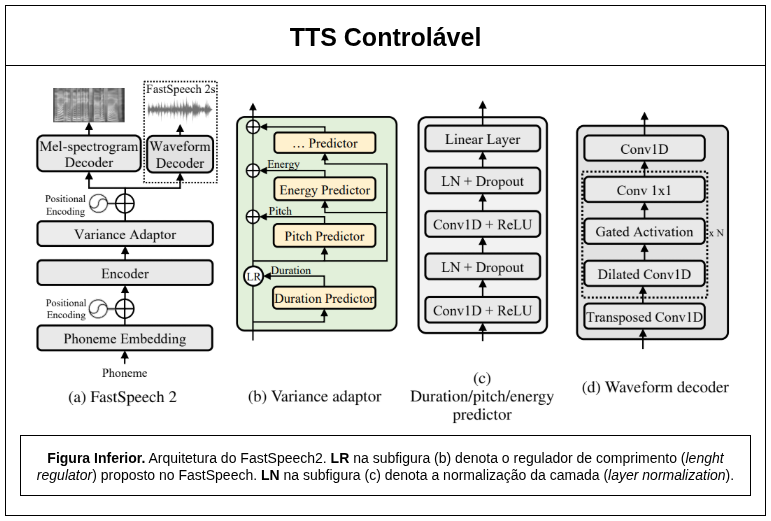
\includegraphics[width=0.7\linewidth]{imgs/DiaTTS-Toolkit-Controllable.png}
    \caption{\textit{FastSpeech2} (\textit{NAR}) baseado em \textit{Transformer} --
    Adaptado de \cite{FastSpeech2}.}
    \label{fig:controllable}
    % \fautor
  \end{figure}
\end{frame}

\begin{frame}{Tipos de modelos de \textit{TTS}}{Difusão vs.\ LLM}
  \setbeamercolor{caption}{bg=white}

  \setbeamertemplate{caption}{
    \begin{beamercolorbox}[wd=\linewidth, center, sep=2pt]{caption}
      {\usebeamercolor[fg]{caption name}\insertcaptionname:} \insertcaption
    \end{beamercolorbox}
  }

  \begin{figure}
    \centering
    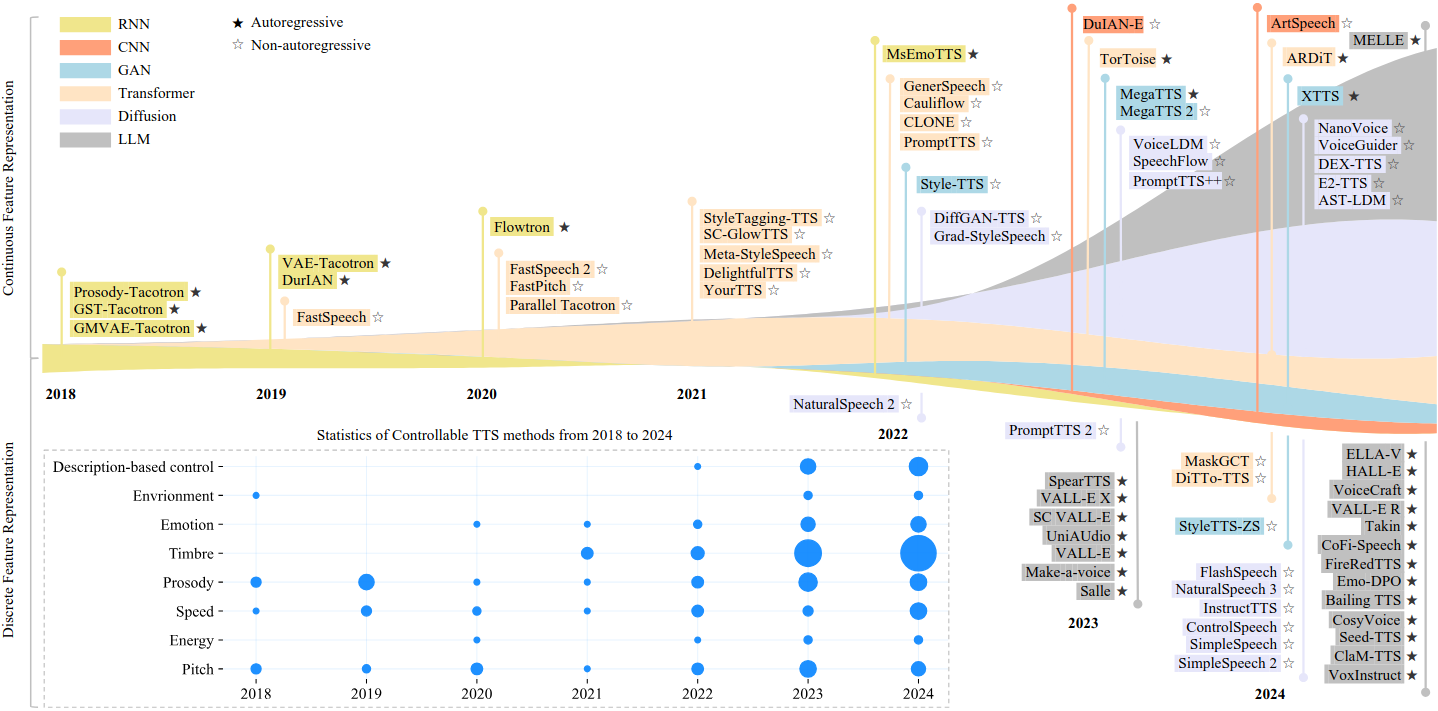
\includegraphics[width=0.8\linewidth]{imgs/SurveyDiffusionLLM.png}
    \caption{Tendência observada da predominância de modelos baseados em \textbf{Difusão}
    e \textbf{LLM} \cite{Survey-ControllableSpeechSynthesis}}.
    \label{fig:diffusion_llm}
  \end{figure}
\end{frame}

% \begin{frame}{Tipos de modelos de \textit{TTS}}{Autorregressivos vs.\ Não-Autorregressivos}
% \begin{block}{Modelos Autorregressivos}
%     \textbf{Definição}
% \end{block}
% \end{frame}

% \begin{frame}{Tipos de modelos de \textit{TTS}}{Autorregressivos vs.\ Não-Autorregressivos}
% \begin{block}{Modelos Não-Autorregressivos}
%     \textbf{Definição}
% \end{block}
% \end{frame}

\begin{frame}{Tipos de modelos de \textit{TTS}}{Sensibilidade ao Diálogo}
  \setbeamercolor{caption}{bg=white}

  \setbeamertemplate{caption}{
    \begin{beamercolorbox}[wd=\linewidth, center, sep=2pt]{caption}
      {\usebeamercolor[fg]{caption name}\insertcaptionname:} \insertcaption
    \end{beamercolorbox}
  }

  \begin{figure}
    \centering
    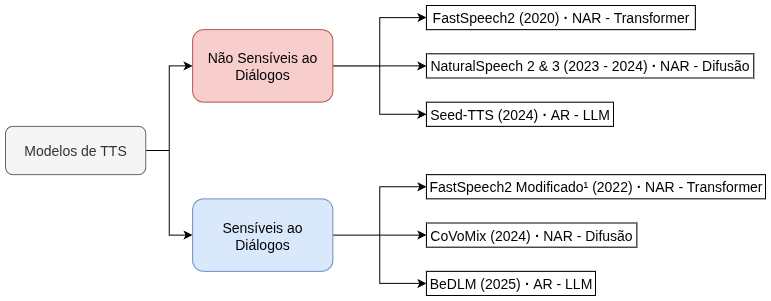
\includegraphics[width=1\linewidth]{imgs/DiaTTS-Toolkit-TTSTypes-AR-NAR.png}
    \caption{Classificação de modelos de TTS quanto ao suporte \textbf{nativo} ao
    diálogo. Fonte: Elaborada pelo autor.}
    \label{fig:tts-dialogue-types}
  \end{figure}
\end{frame}

\begin{frame}{Tipos de modelos de \textit{TTS}}{Sensibilidade ao Diálogo}
  \begin{block}{}
    Os modelos de síntese de fala ainda enfrentam problemas para lidar com a síntese de
    diálogos \cite{Behavior-SD}.
  \end{block}
  \begin{block}{}
    Dentre os modelos sensíveis ao diálogo, nem todas as \textbf{características
    intrínsecas ao diálogo} são capturadas.
  \end{block}
\end{frame}

\begin{frame}{Métricas de Avaliação de Áudios Sintetizados}{Métricas Subjetivas
  vs.\ Métricas Objetivas}
  \begin{block}{Métricas Subjetivas}
    A \textbf{avaliação subjetiva} refere-se a configurações de avaliação nas quais
    \textit{humanos} medem ou quantificam o desempenho e a qualidade \cite{itsp2022_book}.
  \end{block}
  \begin{block}{Métricas Objetivas}
    A \textbf{avaliação objetiva} avalia quantitativamente propriedades acústicas,
    inteligibilidade e similaridade de forma objetiva, sem intervenção de ouvintes
    humanos \cite{itsp2022_book}.
  \end{block}
\end{frame}

\begin{frame}{Métricas de Avaliação de Áudios Sintetizados}{Métricas Subjetivas}
  \begin{block}{MOS}
    \textbf{MOS (\textit{Mean Opinion Score)}:} Mede a qualidade geral e a naturalidade
    intrínseca da voz em uma escala absoluta. É a métrica mais frequente em avaliações
    subjetivas \cite{prosody_eval_julio}.
  \end{block}
\end{frame}

\begin{frame}{Métricas de Avaliação de Áudios Sintetizados}{Métricas Subjetivas}
  \begin{block}{CMOS}
    \textbf{CMOS (Comparative Mean Opinion Score):} Avalia a preferência e a qualidade de
    forma comparativa entre duas amostras de fala \cite{prosody_eval_julio}.
  \end{block}
\end{frame}

\begin{frame}{Métricas de Avaliação de Áudios Sintetizados}{Métricas Subjetivas}
  \begin{block}{EyeTracking-MOS}
    Evolução moderna do \textit{MOS} tradicional \cite{EyetrackingMOS}.
    \begin{itemize}
      \item Maior ``assertividade'' na pontuação devido ao rastreamento ocular.
      \item Aumento significativo na escala do resultado obtido (de $[1 \to 5]$
        para $[0 \to 100]$).
    \end{itemize}
  \end{block}
\end{frame}

\begin{frame}{Métricas de Avaliação de Áudios Sintetizados}{Métricas Objetivas}
  \begin{block}{WER e CER}
    \textbf{WER} (\textit{Word Error Rate}) e \textbf{CER} (\textit{Character Error
    Rate}): Medem a inteligibilidade do áudio sintetizado, submetendo-o a um modelo
    \textit{ASR} e calculando a taxa de erro de palavras e caracteres
    \cite{lang_processing_book}. Fórmula:
    $$WER = \frac{S + D + I}{N}$$
    Onde $S$ representa as substituições, $D$ as deleções, $I$ as inserções e $N$ o
    número total de palavras (ou caracteres, no caso do CER) presentes na referência.
  \end{block}
\end{frame}

\begin{frame}{Métricas de Avaliação de Áudios Sintetizados}{Métricas Objetivas}
  \begin{block}{F0-RMSE}
    \textbf{F0 RMSE} (Raiz do Erro Quadrático Médio da Frequência Fundamental): Avalia a
    precisão do \textit{pitch} e a fidelidade acústica da prosódia. É a métrica objetiva
    mais utilizada na literatura \cite{prosody_eval_julio}. Fórmula:
    $$RMSE_{F0} = \sqrt{\frac{1}{T} \sum_{t=1}^{T} (F0_t - \hat{F0}_t)^2}$$
    Em que $T$ é o número total de quadros, $F0_t$ é a frequência fundamental de
    referência e $\hat{F0}_t$ é a frequência fundamental estimada no quadro $t$.
  \end{block}
\end{frame}

\begin{frame}{Métricas de Avaliação de Áudios Sintetizados}{Métricas Objetivas}
  \begin{block}{TTSDS2- ICLR 2026}
    \textbf{TTSDS2} (\textit{Text-to-Speech Distribution Score 2}) \cite{TTSDS2} é uma
    métrica objetiva, distribucional e multifatorial proposta para avaliar sistemas de
    TTS (\textit{Text-to-Speech}), comparando distribuições de atributos perceptuais da
    fala sintética com a fala real e com distribuições de ruído.
  \end{block}
\end{frame}

\begin{frame}{Métricas de Avaliação de Áudios Sintetizados}{Métricas Objetivas}
  \begin{block}{TTSDS2}
    Fatores:
    \begin{itemize}
      \item \textbf{Genérico} (\textit{generic})
      \item \textbf{Falante} (\textit{speaker})
      \item \textbf{Prosódia} (\textit{}{prosody})
      \item \textbf{Inteligibilidade} (\textit{intelligibility})
    \end{itemize}
    Cálculo da métrica:
    \[
      \text{TTSDS2}(D, \tilde{D}, \mathfrak{D}^{\text{NOISE}}) = 100 \times
      \frac{W_2^\text{NOISE}}{W_2^\text{REAL} + W_2^\text{NOISE}}
    \]
  \end{block}
\end{frame}
